\section{Discussion}
\todo{Intro?}

\subsection{Result of the terrain generation}
The system we have created is capable of generating digital landscapes containing rivers, smaller vegetation, and larger trees. The different components are connected to each other without overlapping, but they still create a visually solid environment.
In the environments created during testing, which represents a forested area, the generation terrain does not require large inclines, but it still results in a landscape that is not fully flat.
The generation of the river results in rivers that curve throughout the terrain, but the planning of the rivers does not work properly. Randomly placing points often results in rivers that generate mostly near the corners of the terrain and are not visible to the camera.
The placement of vegetation allows different types of plants to be placed on the terrain without overlap with each other or with rivers. The distribution can be configured to modify how plants spread or clutter in the environment.

The system is able to generate environments quickly enough. Running the testing setup, the system takes an average of 2.23 seconds to generate an environment with terrain, a single river, and vegetation. Further optimizations can improve this, but when only a small number of environments need to be generated, the current runtime is good enough.

%500 samples
%avg: 2.2303s
%stdev: 0.1332

% Discuss the architecture.
\subsection{Architecture}
In the architecture that we have defined, we have separated the different tasks of generating each terrain feature into one or multiple different components. Each of the components generates, transforms or combines parts of the system. Some of the components are separate to most others, such as the curve planner and fat curve generator, while others are used by a lot of different components, such as the cached intersections between fat curves and chunks.

The different components of the system can be divided into 3 categories, based on the different terrain features. The division of these categories is shown in figure \ref{fig:discussion-architecture-categories}. The first category, category A, is related to the generation of the terrain and the smallest category. Only the generation of the chunks is required to create the terrain. The second category, category B, is responsible for the planning and generating of the rivers, as well as combining the rivers onto the terrain. Category C is used to calculate the positions of objects to be placed onto the terrain using both the PDD and deformation field placement methods. This category depends on both categories, as it requires the heightmap of the chunks to place objects, and uses the rivers to filter object placements. In the figure, the intersections between fat curves and chunks are not divided into a category, since they are used for both category B and C.

% Todo: show why the categories make sense

\begin{figure}
    \centering
    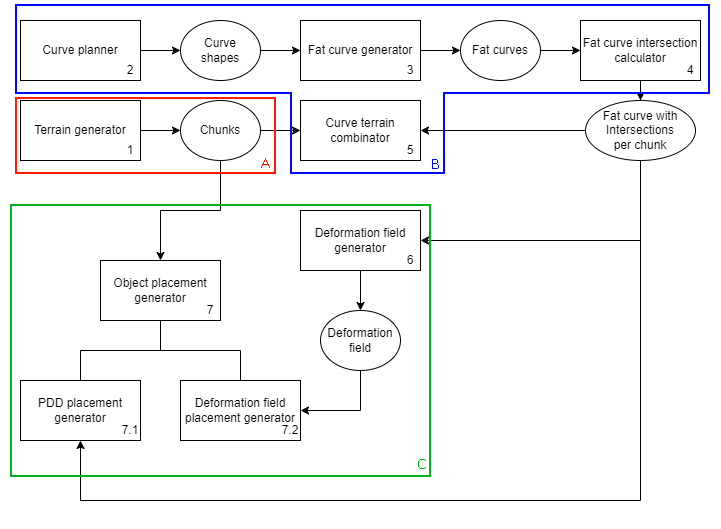
\includegraphics[width=\linewidth]{figures/architecture/Architecture-categories.png}
    \caption{Architecture of the system with components categorised for each environment feature}
    \label{fig:discussion-architecture-categories}
\end{figure}

% Discuss validation: PDD density
\subsection{Parameters of the system}
For each of the components in the system, we have established a set of parameters that influence the generated terrain. Some of these parameters, such as the size and resolution of the height maps of the terrain, can be kept constant for any generated terrain. With the other parameters, the user is able to influence the generated terrain. 
%A list of all parameters separated in these two categories can be found in appendix \ref{appendix:parameters}.

For the parameters related to the generation of the terrain, most of the parameters are very technical. The parameters of the fractal noise algorithm are mainly mathematical and are not accessible for users without experience with noise functions. Due to this, when a designer wants a specific feature on the terrain, more experimentation is required to generate a terrain that is acceptable to the user.

To plan the generation of the river, the parameters used have a clearer meaning to how they influence the system. The planned rivers follow a specific pattern, namely a meandering curve that can change directions randomly, and the parameters can influence the pattern the river takes. Differences to the amplitude of the meandering or the random rotation maximum can result in different characteristics of rivers, as shown in the research by Teoh \cite{teoh_riverland_2009}. In the current version of the system, there are no direct parameters that contribute to the initial position and direction of the river, so this is still a completely random process.
To transform the river path into a fat curve, the process mainly contains constant parameters. Since the interpolation of the path uses Bezier curves, a parameter has been added to derive the tangents of each control point. As this is mainly to control the smoothing of the curve, this parameter can be kept as a constant.

The parameters related to placing objects are closely related to the type of vegetation used. For the PDD algorithm, the parameters are related to the physical size of the objects that need to be placed. For trees, these are the outer radius which equates to the size of the canopy, which prevents overlap between trees, and the inner radius, which is to prevent overlap with smaller objects. In testing multiple layers of PDD placement have not beeen used, but the inner radius is still required for creating an initial deformation field for the second step of placing objects.

Before objects are placed using the deformation kernel method, the initial deformation field is generated. On this initial field the rivers and PDD objects are placed, to filter locations where plants cannot be placed. To allow for certain plants to be generated near or away of rivers, there are parameters that select the initial probability based on the fat curves. For PDD objects, the area within the inner radius of the PDD object is completely removed to avoid overlap between the two objects.

\todo{Deformation kernel itself}

\subsection{Validating system components}
To validate the generated terrain, we have used a number of different metrics to check and control the environment. Each of these methods analyses a specific component and how it affects the generated environment. Currently, these methods are not directly involved in the final terrain generation, but can instead be used after a terrain has been generated to improve the result.

% PDD density
For the placement of PDD objects, we have experimented with increasing the outer radius to reduce the density of trees. From this, we see an inverse relation between the radius of the object and the density of the objects within the area. To find this relation, we fitted two functions on the dataset, the exponential function and an inverse quadratic relation. These fits are shown in figure \ref{fig:discussion-pdd-graph}. For both fits, we calculated the mean squared error, which is shown in table \ref{tab:discussion-pdd-mse}. From this we can see that the quadratic relation has a better fit. This is expected, since increasing the radius linearly results in the area quadratically, which results in a quadratic decrease in the amount of points that can be placed. With this relation, the user has an indication of the expected density of the objects generated.

\begin{figure}
    \centering
    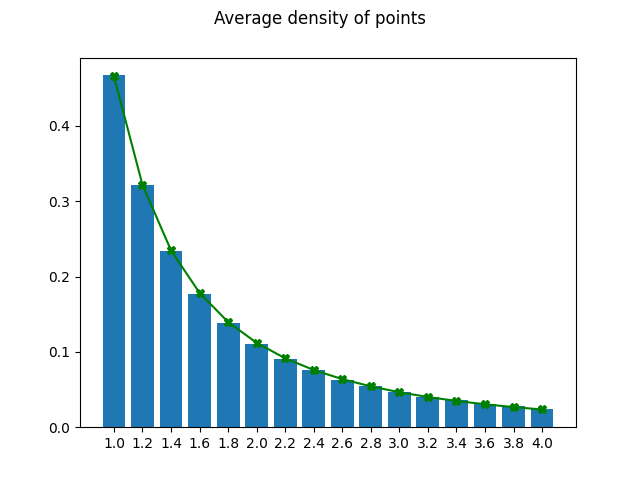
\includegraphics[width=0.5\linewidth]{figures/parameters/pdd-parameters-graph-fit.png}
    \caption{The density of points with varying ratios, with an exponential and inverse quadratic fit}
    \label{fig:discussion-pdd-graph}
\end{figure}

\begin{table}[h]
    \centering
    \begin{tabular}{|c|c|}
        \hline
        Function & MSE \\
        \hline
        Exponential & $3.97 * 10^{-5}$  \\
        Quadratic & $9.60 * 10^{-7}$ \\
        \hline
    \end{tabular}
    \caption{Mean squared error of different relations.}
    \label{tab:discussion-pdd-mse}
\end{table}

\subsubsection{River visibility}
In the current implementation of the system, generating a river that is visible is very unreliable. Since the start point and direction of the rivers are selected randomly, rivers often only traverses for a small distance before moving out of bounds or travels near a border that is not visible from the perspective of the camera. In the initial version more than 80\% of all rivers has a visibility of lower than 5\% of the total terrain surface, which results in a large number of terrains to be generated before an acceptable terrain appears. Improving this method by taking multiple camera positions into account has improved the system somewhat, although there is still a large proportion of all generated rivers that still does not contain a large section of the river. If a river is generated near the corner of the terrain, none of the camera positions will be able to view the river.

\subsubsection{Single object occlusion}
To validate whether the view is obscured by a large single object, we have used panoptic segmentation to calculate the size of each object in the view. With this, we found that the system sometimes generates objects close to the camera that take up almost all space in the view (Figure \ref{fig:single-object-large}).

The solution to remove all objects close to the camera has resulted in removing most large objects in the view. A few examples of terrains generated using this method are shown in Figure \ref{fig:discussion-tree-visibility-improved-examples}. Although the second rounds of experiments still contained objects that cover more than 30\% of the view, the large majority of views do not contain a large object in front of the camera. Although this approach seems to work well when looking at the statistics, the types of environment generated do look more sparse due to the empty space between the camera and the first trees. When generating a more dense environment, this approach removes a large part of this density.

\begin{figure}
    \begin{subfigure}{.5\textwidth}
        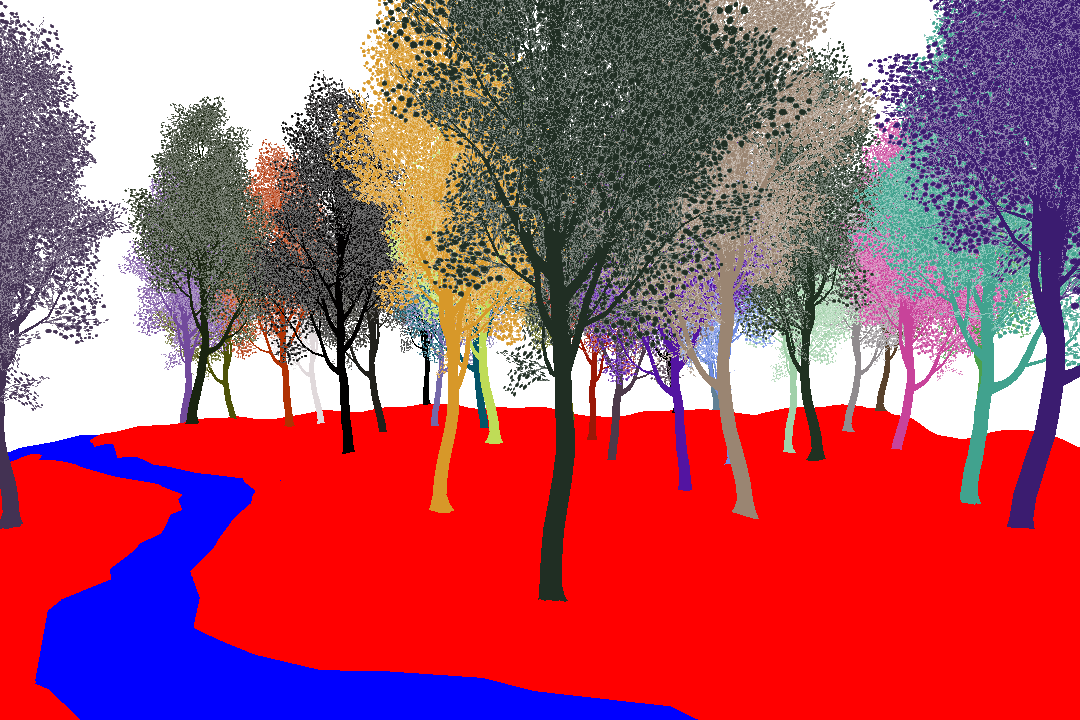
\includegraphics[width=\linewidth]{figures/validation/tree-visibility-improved-1.png}
    \end{subfigure}
    \begin{subfigure}{.5\textwidth}
        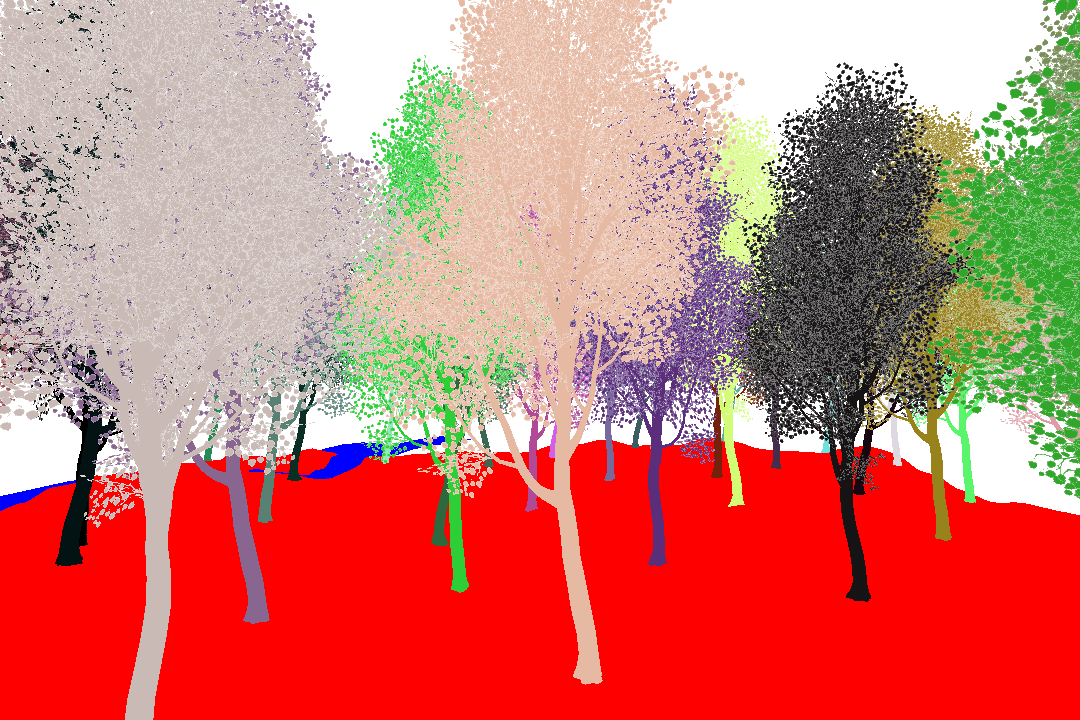
\includegraphics[width=\linewidth]{figures/validation/tree-visibility-improved-2.png}
    \end{subfigure}
    \caption{Examples of environments generated with objects closer than 11 units removed}
    \label{fig:discussion-tree-visibility-improved-examples}
\end{figure}
